\chapter{Dados abertos}

Os dados são disponibilizados, semestralmente, em planilhas baseadas no modelo da
Figura \ref{fig:modelo_prf}, e para obter dados específicos de cada acidente, as informações precisam ser
correlacionadas entre tabelas, que podem ser vistas na Figura \ref{fig:tabela_dados}. As planilhas também contêm
uma grande quantidade de dados, pois são divulgados cerca de 45.000 acidentes por semestre,
além de uma quantidade exagerada de tabelas para o relacionamento, pouco eficiente, dos
dados.

\begin{figure}[!htb]
 \centering
 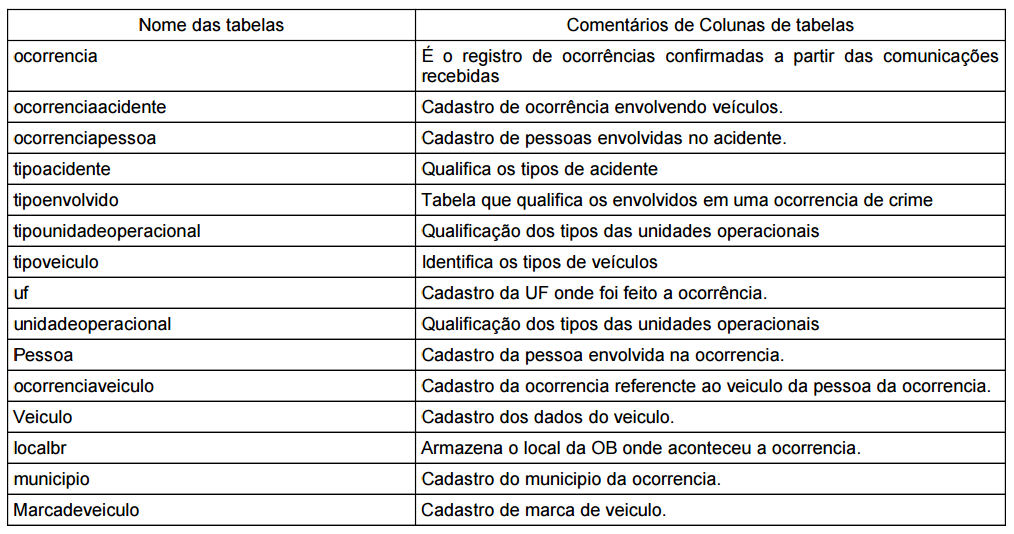
\includegraphics[scale = 0.4]{tabela_dados}
 \caption[Tabelas da base de dados da PRF]{Tabelas da base de dados da PRF. Fonte: \cite{brasil13}}
 \label{fig:tabela_dados}
\end{figure}

\begin{figure}[!htb]
 \centering
 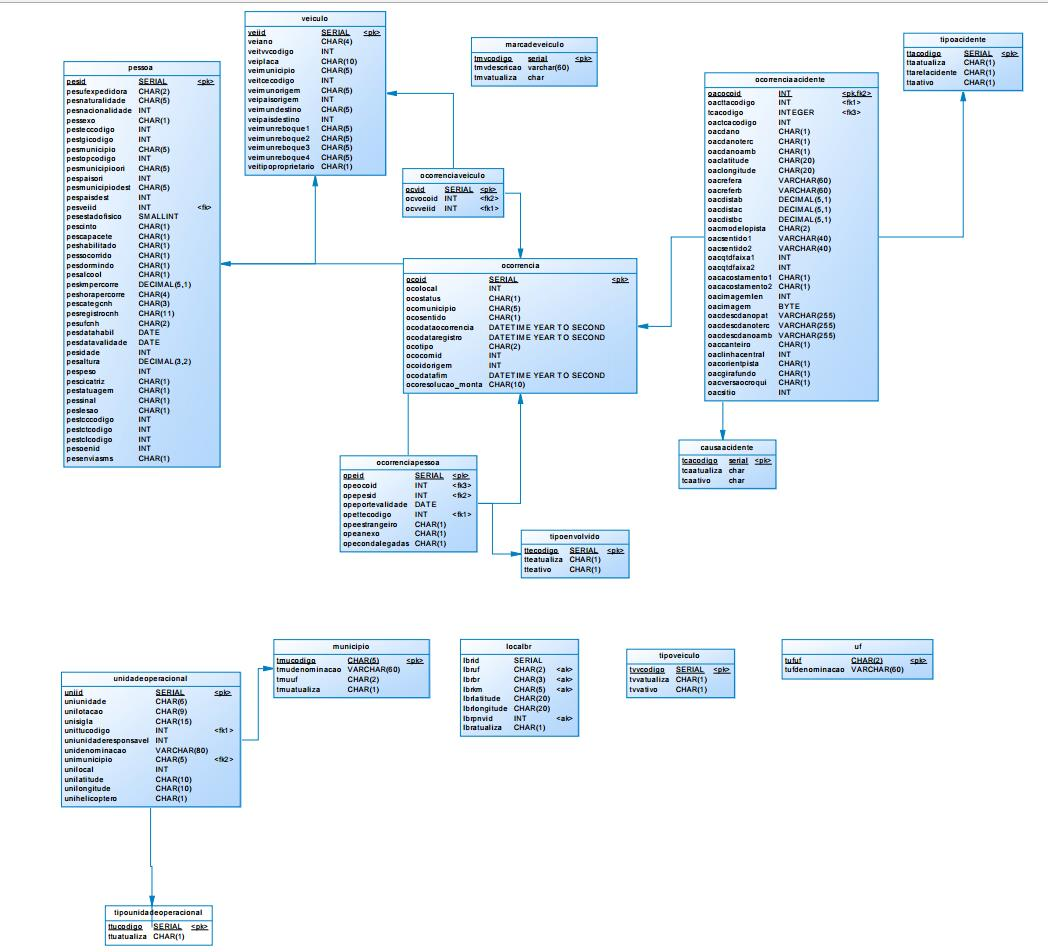
\includegraphics[scale = 0.4]{modelo_prf}
 \caption[Modelo de Dados atual das Ocorrências de Acidentes em Rodovias Federais]
  {Modelo de Dados atual das Ocorrências de Acidentes em Rodovias Federais. Fonte: \cite{brasil13}}
 \label{fig:modelo_prf}
\end{figure}

\vfill